\documentclass[
	% -- opções da classe memoir --
	12pt,				% tamanho da fonte
	openright,			% capítulos começam em pág ímpar (insere página vazia caso preciso)
	oneside,			% para impressão em apenas anverso. Oposto a twoside
	%twoside,			% para impressão em verso e anverso. Oposto a oneside
	a4paper,			% tamanho do papel. 
	% -- opções da classe abntex2 --
	%chapter=TITLE,		% títulos de capítulos convertidos em letras maiúsculas
	%section=TITLE,		% títulos de seções convertidos em letras maiúsculas
	%subsection=TITLE,	% títulos de subseções convertidos em letras maiúsculas
	%subsubsection=TITLE,% títulos de subsubseções convertidos em letras maiúsculas
	% -- opções do pacote babel --
	english,			% idioma adicional para hifenização
	francais,			% idioma adicional para hifenização
	spanish,			% idioma adicional para hifenização
	brazil				% o último idioma é o principal do documento
	]{abntex2}

% Evita linhas orfãs e viúvas
\widowpenalty=10000
\clubpenalty=10000

\usepackage{lmodern}			% Usa a fonte Latin Modern
\usepackage[T1]{fontenc}		% Selecao de codigos de fonte.
\usepackage[utf8]{inputenc}		% Codificacao do documento (conversão automática dos acentos)
\usepackage{lastpage}			% Usado pela Ficha catalográfica
\usepackage{indentfirst}		% Indenta o primeiro parágrafo de cada seção.
\usepackage{color}				% Controle das cores
\usepackage{graphicx}			% Inclusão de gráficos
\usepackage{microtype} 			% para melhorias de justificação
\usepackage{lipsum}				% para geração de dummy text
\usepackage[brazilian,hyperpageref]{backref}	% Paginas com as citações na bibl
\usepackage[alf]{abntex2cite}					% Citações padrão ABNT
\usepackage{graphicx}
\usepackage{tikz}
\usetikzlibrary{shapes,arrows,chains}
\usepackage[]{mcode}
\usepackage{multirow}
\usepackage{array}
\usepackage{longtable}
\usepackage{rotating}
\usepackage{caption}

\addto\captionsbrazil{
	%% ajusta nomes padroes do babel
	\renewcommand{\bibname}{Refer\^encias}
	\renewcommand{\indexname}{\’Indice Remissivo}
	\renewcommand{\listfigurename}{Lista de Figuras}
	\renewcommand{\listtablename}{Lista de Tabelas}
	\renewcommand{\listadesiglasname}{Lista de Abreviaturas e Siglas}
	%% ajusta nomes usados com a macro \autoref
	\renewcommand{\pageautorefname}{p\’agina}
	\renewcommand{\sectionautorefname}{se{\c c}\~ao}
	\renewcommand{\subsectionautorefname}{subse{\c c}\~ao}
	\renewcommand{\paragraphautorefname}{par\’agrafo}
	\renewcommand{\subsubsectionautorefname}{subse{\c c}\~ao}
}

% ---
% Configurações do pacote backref
% Usado sem a opção hyperpageref de backref
\renewcommand{\backrefpagesname}{Citado na(s) página(s):~}
% Texto padrão antes do número das páginas
\renewcommand{\backref}{}
% Define os textos da citação
\renewcommand*{\backrefalt}[4]{
	\ifcase #1 %
		Nenhuma citação no texto.%
	\or
		Citado na página #2.%
	\else
		Citado #1 vezes nas páginas #2.%
	\fi}%
% ---

\definecolor{blue}{RGB}{0,114,189}
\definecolor{orange}{RGB}{217,83,25}
\definecolor{yellow}{RGB}{237,177,32}
\definecolor{purple}{RGB}{126,47,142}
\definecolor{green}{RGB}{119,172,48}
\definecolor{lightBlue}{RGB}{77,190,238}
\definecolor{red}{RGB}{162,20,47}
\definecolor{black}{RGB}{0,0,0}

% informações do PDF
\makeatletter
\hypersetup{
     	%pagebackref=true,
		pdftitle={\@title}, 
		pdfauthor={\@author},
    	pdfsubject={\imprimirpreambulo},
	    pdfcreator={LaTeX with abnTeX2},
		pdfkeywords={abnt}{latex}{abntex}{abntex2}{trabalho acadêmico}, 
		colorlinks=true,	% false: boxed links; true: colored links
    	linkcolor=black,	% color of internal links
    	citecolor=black,	% color of links to bibliography
    	filecolor=black,	% color of file links
		urlcolor=black,
		bookmarksdepth=4
}
\makeatother

% --- 
% Espaçamentos entre linhas e parágrafos 
% --- 
% O tamanho do parágrafo é dado por:
\setlength{\parindent}{1.3cm}
% Controle do espaçamento entre um parágrafo e outro:
\setlength{\parskip}{0.2cm}  % tente também \onelineskip


\titulo{Métodos de Segmentação Automática de Sinais de Eletromiografia de Superfície para Classificação de Movimentos Utilizando Redes Neurais Artificiais}
\autor
{
	UNIVERSIDADE FEDERAL DO RIO GRANDE DO SUL\\
	ESCOLA DE ENGENHARIA\\
	DEPARTAMENTO DE ENGENHARIA ELÉTRICA\\
	GRADUAÇÃO EM ENGENHARIA ELÉTRICA\\
	\vspace*{4\baselineskip} 
	VICENTE COSTAMILAN DA CUNHA
}
\local{Porto Alegre}
\data{2015}
\orientador{Prof. Dr. Eng. Alexandre Balbinot}
\coorientador{}
\instituicao{}
\tipotrabalho{Monografia (graduação)}
% O preambulo deve conter o tipo do trabalho, o objetivo, 
% o nome da instituição e a área de concentração 
\preambulo{Projeto de Diplomação apresentado ao Departamento de Engenharia Elétrica da Escola de Engenharia da Universidade Federal do Rio Grande do Sul, como requisito parcial para Graduação em Engenharia Elétrica}

% --- 

% ---
% compila o indice
% ---
\makeindex
% ---

\begin{document}
\selectlanguage{brazil}
\frenchspacing 
\imprimircapa
\imprimirfolhaderosto*

%=========================================================================
% FOLHA DE APROVAÇÃO
%=========================================================================

\begin{folhadeaprovacao}

  \begin{center}
    {\ABNTEXchapterfont\large\imprimirautor}

    \vspace*{\fill}\vspace*{\fill}
    \begin{center}
      \ABNTEXchapterfont\bfseries\Large\imprimirtitulo
    \end{center}
    \vspace*{\fill}
    
    \hspace{.45\textwidth}
    \begin{minipage}{.5\textwidth}
        \imprimirpreambulo
    \end{minipage}%
    \vspace*{\fill}
   \end{center}
        
   Trabalho aprovado. \imprimirlocal, XX de XXXXXX de 2015:

   \assinatura{\textbf{\imprimirorientador} \\ Orientador} 
   \assinatura{\textbf{Professor} \\ Convidado 1}
   \assinatura{\textbf{Professor} \\ Convidado 2}
   %\assinatura{\textbf{Professor} \\ Convidado 3}
   %\assinatura{\textbf{Professor} \\ Convidado 4}
      
   \begin{center}
    \vspace*{0.5cm}
    {\large\imprimirlocal}
    \par
    {\large\imprimirdata}
    \vspace*{1cm}
  \end{center}
  
\end{folhadeaprovacao}

%=========================================================================
% DEDICATÓRIA
%=========================================================================

\begin{dedicatoria}
   \vspace*{\fill}
   \centering
   \noindent
   \textit{ A Gilberto, mi padre, torre de razón y de firme fe; \\ e a todos aqueles que tomarem interesse neste estudo.} \vspace*{\fill}
\end{dedicatoria}

%=========================================================================
% AGRADECIMENTOS
%=========================================================================

\begin{agradecimentos}
	Aos demais colaboradores e pesquisadores do laboratório de Instrumentação Eletro-Eletrônica, em especial Vinicius Cene e Fernanda Trevisol, que desenvolveram a coleta da base de dados utilizada e prestaram auxílio de forma geral.
\end{agradecimentos}

%=========================================================================
% EPÍGRAFE
%=========================================================================

\begin{epigrafe}
    \vspace*{\fill}
	\begin{flushright}
		\textit{Take nothing on its looks;\\ take everything on evidence.\\ There's no better rule.}\\ \vspace{\onelineskip}
		Charles Dickens, Great Expectations
	\end{flushright}
\end{epigrafe}

%=========================================================================
% RESUMOS
%=========================================================================

% resumo em português
\setlength{\absparsep}{18pt} % ajusta o espaçamento dos parágrafos do resumo
\begin{resumo}

	A segmentação de sinais de eletromiografia (EMG) é parte essencial de preprocessamento em aplicações de reconhecimento de movimentos e controle de próteses, separando trechos de interesse do sinal correspondentes a esforços musculares e descartando trechos de sinal com baixa atividade muscular. Neste estudo, quatro métodos para segmentação automática de sinais de EMG foram implementados em MATLAB. Os métodos foram aplicados aos sinais de EMG de superfície a base de dados do projeto NinaPro e aos sinais da base de dados adquiridos pelo Laboratório de Instrumentação Eletro-Eletrônica da UFRGS. Redes neurais artificais (RNAs) foram utilizadas para classificar os movimentos realizados relativos aos sinais segmentados com os quatro métodos. \textcolor{red}{TODO: RESULTADOS}.

	\vspace{\onelineskip}
	\textbf{Palavras-chave}: Eletromiografia. Segmentação. Base de dados NinaPro. Redes Neurais Artificiais.
\end{resumo}

% resumo em inglês
\begin{resumo}[Abstract]
 \begin{otherlanguage*}{english}
	\textcolor{red}{TODO: TRADUZIR RESUMO}.
	
   \vspace{\onelineskip}
   \noindent 
   \textbf{Keywords}: Eletromiography. Segmentation. MATLAB. NinaPro database. Artificial Neural Networks.
 \end{otherlanguage*}
\end{resumo}

%=========================================================================
% SUMÁRIOS
%=========================================================================

% inserir lista de ilustrações
\pdfbookmark[0]{\listfigurename}{lof}
\listoffigures*
\cleardoublepage

% inserir lista de tabelas
\pdfbookmark[0]{\listtablename}{lot}
\listoftables*
\cleardoublepage

% inserir lista de abreviaturas e siglas
\begin{siglas}
  	\item[EMG]		Eletromiografia
	\item[NinaPro]	\emph{Non-Invasive Adaptive Prosthetics project}
	\item[MU]		\emph{Motor Unit}
  	\item[MUAP]		\emph{Motor Unit Action Potencial}
	\item[MUAPT]	\emph{Motor Unit Action Potencial Trains}
	\item[MTD\#]	\emph{Método número \#}
	\item[BEP]		\emph{Beginning Extraction Point}
	\item[EEP]		\emph{Ending Extraction Point}
\end{siglas}

% inserir o sumario
\pdfbookmark[0]{\contentsname}{toc}
\tableofcontents*
\cleardoublepage

\textual
%=========================================================================
% INTRODUÇÃO
	\chapter{Introdução}
%=========================================================================
Sinais de EMG apresentam crescentes aplicações no controle de próteses mioelétricas. Por exemplo, \cite{Hargrove2013} mostra o controle de uma prótese de perna de um amputado acima do joelho direito, enquanto \cite{Jun-UkChu2007} apresentou bons resultados de reconhecimento de padrões de EMG para desenvolvimento de uma prótese multifuncional de mão. Utilizando redes neurais artificiais, \cite{Pattichis1995} mostra realização de diagnósticos clínicos de desordens neuromusculares em sinais de EMG invasivo (adquirido por agulhas).

As principais estratégias para caracterização de sinais de EMG e potenciais de ação das unidades motoras baseiam-se no uso de um método classificador. Métodos de classificação utilizados incluem - entre inúmeros outros - redes neurais artificiais \cite{Hudgins1993}, classificador Bayesiano \cite{Englehart2003} e lógica \emph{fuzzy} \cite{Chan2000}. Tais sistemas de classificação necessitam, como parte do preprocessamento, segmentar os sinais de EMG adquiridos, para então realizar extração de características dos segmentos como amplitude, número de cruzamentos por zero, coeficientes de autoregressão, transformadas de Fourier e, mais recentemente, transformadas Wavelet \cite{Jun-UkChu2007}. 

Neste trabalho, propõe-se e implementa-se em MATLAB quatro diferentes métodos de segmentação automática para sinais de EMG de superfície. Os primeiros dois métodos (que serão identificados neste estudo pelas abreviações MTD1 e MTD2) tratam da detecção de picos do sinal utilizando \emph{thresholding} e produzem segmentos de comprimento constante centrados nestes picos. O terceiro (MTD3) e quarto (MTD4) métodos utilizam de janela deslizante para identificação de pontos iniciais e finais dos segmentos, produzindo segmentos de comprimento variável.

O primeiro método (MTD1) é baseado no método de segmentação utilizado em \cite{Chauvet2001}. Trata-se de método iterativo, identificando os picos do sinal a partir de \emph{threshold} de amplitude, segmentando o sinal em janelas de comprimento constante centradas nos picos. O valor de \emph{threshold} para a primeira iteração corresponde ao máximo absoluto do sinal. A cada nova iteração em que não se atinge um número desejado de segmentos, o novo \emph{threshold} é calculado como fração do \emph{threshold} da iteração anterior.

O segundo método (MTD2) é baseado no método de segmentação utilizado em \cite{Katsis2006}. De forma similar ao MTD1, também utiliza \emph{threshold} para detecção de picos do sinal e segmentação com janelas de comprimento constante em torno dos picos. Diferentemente de MTD1, MTD2 não é iterativo, utilizando relação entre valor máximo e comprimento do sinal para cálculo do valor de \emph{threshold}.

O terceiro método (MTD3) é baseado no método de segmentação utilizado em \cite{Gut2000}. Uma janela deslizante percorre o sinal e identifica inícios de segmentos quando a declividade média no interior da janela excede determinado valor limite. Os finais dos segmentos são identificados quando a variação total do sinal no interior da janela é inferior a um segundo valor de \emph{threshold}.

O quarto método (MTD4) é baseado no método de segmentação utilizado em \cite{Pattichis1995}. Os pontos de início do segmento são tais que, em uma janela à esquerda do ponto, o sinal mantém-se abaixo de determinado \emph{threshold}. Os pontos de final de segmento, de forma similar, são tais que, em uma janela à direita do ponto, o sinal mantém-se abaixo do \emph{threshold}.

Utilizando valores de RMS, variância e frequência mediana dos segmentos obtidos, redes neurais artificiais (RNAs) serão treinadas para classificar entre os 17 diferentes movimentos de mão e punho constantes do exercício 1 da base de dados número 2 do projeto NinaPro \cite{Gijsberts2014}. Os objetivos finais deste trabalho são a implementação dos métodos de segmentação propostos (para possível uso em trabalhos futuros do laboratório de Instrumentação Eletro-Eletrônica) e fornecer avaliação comparativa entre métodos a respeito da taxa de acerto de classificação obtida com uso de RNA.

%=========================================================================
% REVISÃO BIBLIOGRÁFICA
	\chapter{Revisão Bibliográfica}
%=========================================================================
		\section{Sinais de Eletromiografia}
%-------------------------------------------------------------------------
Sinais de EMG podem ser adquiridos por eletrodos posicionados na superfície da pele (eletrodo não invasivo) ou por agulhas introduzidas no tecido muscular (eletrodo invasivo). Os sinais são formados por potenciais de ação de fibras musculares organizadas em unidades funcionais chamadas de ``unidades motoras'' (MU - \emph{Motor Unit}) \cite{Luca2006}. Uma unidade motora é composta por um neurônio motor e as fibras musculares que ele inerva, e é a entidade fundamental que controla a ativação de músculos estriados \cite{Buchthal980}. A soma algébrica dos potenciais de ação de todas as fibras de uma unidade motora é chamada de ``potencial de ação da unidade motora'', ou em inglês, MUAP (\emph{Motor Unit Action Potential}) \cite{Almeida1997}. A Figura \ref{fig_MUAP_comp} apresenta a composição de uma MUAP a partir da soma dos potenciais das fibras de uma unidade motora.

\begin{figure}[htb]
	\caption{\label{fig_MUAP_comp}Soma de potenciais de ação das $n$ fibras de uma unidade motora, formando uma MUAP $h(t)$.}
	\begin{center}
	    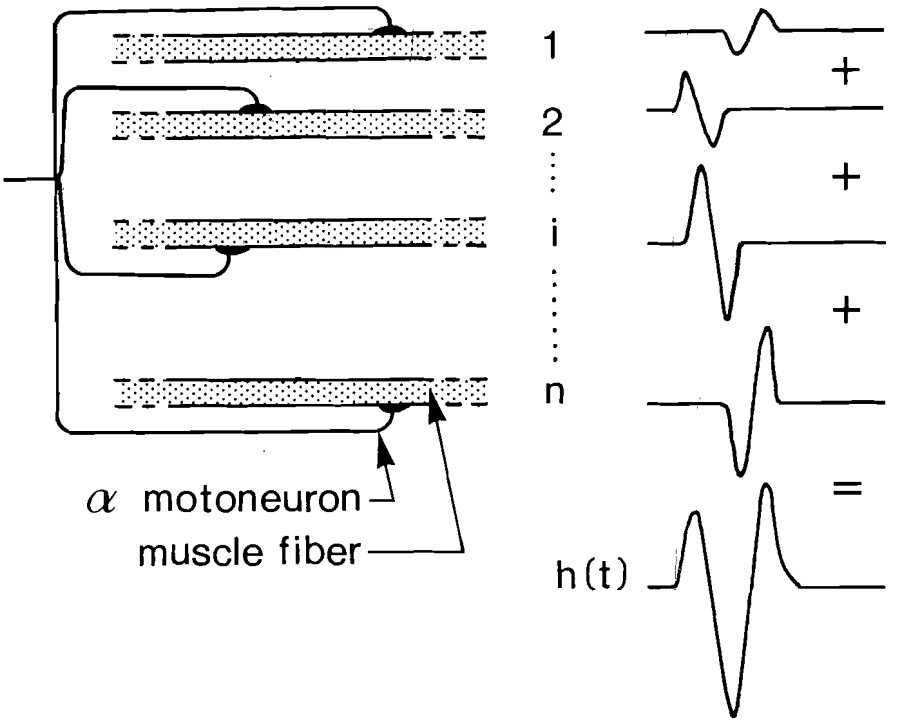
\includegraphics[width=0.75\linewidth]{./img/MUAP_oneMU.png}
	\end{center}
	\legend{Fonte: adaptado de \cite{Basmajian1985}.}
\end{figure}

Dependendo do método utilizado para aquisição de EMG, é comum a captura da contribuição de mais de uma unidade motora no mesmo canal. A influência de uma unidade motora na amplitude sinal adquirido depende principalmente da distância das fibras musculares ao ponto de aquisição \cite{Gerdle1999}. Sinais de EMG de longa duração são constituídos por sequências temporais de MUAPs, também conhecidas como MUAPTs (\emph{MUAP Trains}). A Figura \ref{fig_MUAP_trains} exemplifica MUAPTs de diferentes MUs que somam-se para formar um sinal de EMG de longa duração.

\begin{figure}[htb]
	\caption{\label{fig_MUAP_trains}MUAPTs de diferentes MUs somam-se para compor o sinal adquirido por um canal de EMG.}
	\begin{center}
	    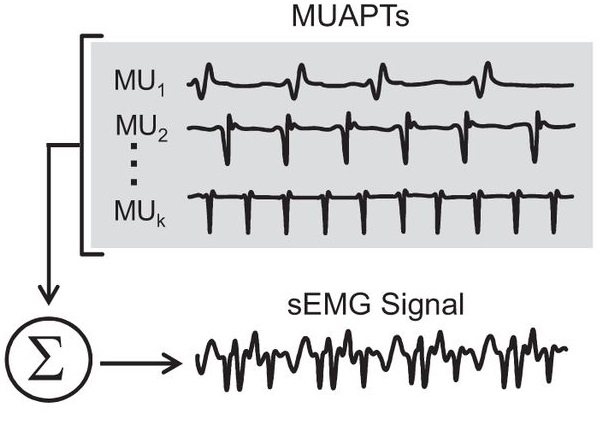
\includegraphics[width=0.75\linewidth]{./img/MUAP_trains.jpg}
	\end{center}
	\legend{Fonte: adaptado de \cite{Kline2014}}
\end{figure}

\textcolor{red}{TODO: adicionar referência ao trabalho de Favieiro}.

%-------------------------------------------------------------------------
		\section{Métodos de Segmentação}
%-------------------------------------------------------------------------
\label{sec:MTDs}
Esta seção descreve os métodos de segmentação desenvolvidos neste trabalho, citando os trabalhos da área que foram utilizados como base teórica para os métodos. Nota-se que nomes utilizados para variáveis e constantes (por exemplo, sinal a ser segmentado `$x$', \emph{threshold} `$T$', etc.) foram determinados pelo autor deste trabalho, não necessariamente sendo os mesmos utilizados nos trabalhos citados.

Para as definições dos métodos 3 e 4 (MTD3 e MTD4) são utilizados os termos BEP (\emph{beginning extraction point}, ponto inicial de um segmento) e EEP (\emph{ending extraction point}, ponto final de um segmento), também utilizados em \cite{Pattichis1995}.
	
%-------------------------------------------------------------------------
				\subsection{Método 1 - método iterativo utilizando \emph{thresholding} para detecção de centros de segmentos de comprimento constante (MTD1)}
%-------------------------------------------------------------------------
Este método iterativo é adaptado do método de segmentação utilizado em \cite{Chauvet2001}. As definições da Tabela \ref{tab_mtd1params} serão utilizados para descrever este método.

\begin{table}[htb]
\IBGEtab{%
	\caption{Parâmetros utilizados para definir o MTD1.}%
	\label{tab_mtd1params}
}{%
	\begin{tabular}{ccc}
	\toprule
	Nome & Descrição \\
	\midrule \midrule
	$x$ & Sinal a ser segmentado \\
	\midrule
	$L$ & Comprimento total do sinal a ser segmentado \\
	\midrule
	$l$ & Comprimento desejado para os segmentos \\
	\midrule
	$T_k$ & Valor de \emph{threshold} para a iteração $k$ \\
	\midrule
	$T_{lim}$ & Valor de limite inferior para o \emph{threshold} \\
	\midrule 
	$q$ & Fração de $T_{k-1}$ para determinação de $T_k$ \\
	\midrule 
	$N_{k}$ & Número total de candidatos para centros de segmentos identificados na iteração $k$ \\
	\midrule 
	$r_k$ & Razão entre número de candidatos identificados na iteração $k$ e o comprimento total do sinal \\
	\midrule 
	$r_{target}$ & Razão mínima esperada para $r_k$, utilizada para determinar o final do método \\
	\bottomrule
\end{tabular}%
}{%
}
\end{table}


Inicialmente, determina-se o valor de \emph{threshold} $T_0$ equivalente ao máximo absoluto do sinal a ser segmentado $x$ (Equação (\ref{eq:mtd1t0})). O valor $T_k$ é atualizado em cada iteração $k$ como sendo uma fração $q$ de $T_{k-1}$ (Equação (\ref{eq:mtd1tk})). No trabalho de \cite{Chauvet2001}, este valor $q$ foi empiricamente determinado em 90\%.

\begin{equation}
\label{eq:mtd1t0}
  T_0 = max(x)
\end{equation}

\begin{equation}
\label{eq:mtd1tk}
  T_k = q \times T_{k-1}
\end{equation}

Pontos do sinal acima do valor de $T_k$ são possíveis candidatos para centros de segmentos. Caso exista mais de um possível candidato em uma vizinhança bilateral de $l$ amostras do sinal, apenas o ponto de maior amplitude nesta vizinhança é considerado. Para determinar o final do método, avalia-se a razão $r_k$ entre a quantidade identificada de candidatos $N_{k}$ e o comprimento total do sinal $L$ (equação \ref{eq:mtd1rk}). Caso $r_k$ seja menor que um valor predeterminado $r_{target}$, calcula-se $T_{k+1}$ para realização da próxima iteração (equação \ref{eq:mtd1tk}). Caso $r_k$ seja maior ou igual ao valor predeterminado $r_{target}$, encerra-se o método e os segmentos são tomados como janelas de sinal de comprimento $l$, centradas nos candidatos identificados na última iteração.

\begin{equation}
\label{eq:mtd1rk}
  r_k = \frac{N_{k}}{L} 
\end{equation}

Adicionalmente, o estabelecimento de um valor limite mínimo para \emph{threshold} $T_{lim}$ garante que o método não entre em laço infinito e evita detecção de segmentos em trechos de baixa atividade muscular. Caso o valor de \emph{threshold} $T_k$ para a iteração atual seja inferior a $T_{lim}$, encerra-se o processo iterativo. O método de segmentação MTD1 é representado pelo fluxograma da Figura \ref{fig_mtd1flux}.

% Set up a few colours
\colorlet{lcfree}{green}
\colorlet{lcnorm}{blue}
\colorlet{lccong}{red}
% -------------------------------------------------
% Set up a new layer for the debugging marks, and make sure it is on
% top
\pgfdeclarelayer{marx}
\pgfsetlayers{main,marx}
% A macro for marking coordinates (specific to the coordinate naming
% scheme used here). Swap the following 2 definitions to deactivate
% marks.
\providecommand{\cmark}[2][]{%
  \begin{pgfonlayer}{marx}
    \node [nmark] at (c#2#1) {#2};
  \end{pgfonlayer}{marx}
  } 
\providecommand{\cmark}[2][]{\relax} 
% -------------------------------------------------
% Start the picture
\begin{figure}[htb]
	\caption{\label{fig_mtd1flux}Fluxograma representativo do MTD1.}
	\begin{center}
		\begin{tikzpicture}[%
			>=triangle 60,              % Nice arrows; your taste may be different
			start chain=going below,    % General flow is top-to-bottom
			node distance=6mm and 60mm, % Global setup of box spacing
			every join/.style={norm},   % Default linetype for connecting boxes
			]
		% ------------------------------------------------- 
		% A few box styles 
		% <on chain> *and* <on grid> reduce the need for manual relative
		% positioning of nodes
		\tikzset{
		  base/.style={draw, on chain, on grid, align=center, minimum height=4ex},
		  proc/.style={base, rectangle, text width=8em},
		  test/.style={base, diamond, aspect=2, text width=8em},
		  term/.style={proc, rounded corners},
		  % coord node style is used for placing corners of connecting lines
		  coord/.style={coordinate, on chain, on grid, node distance=6mm and 25mm},
		  % nmark node style is used for coordinate debugging marks
		  nmark/.style={draw, cyan, circle, font={\sffamily\bfseries}},
		  % -------------------------------------------------
		  % Connector line styles for different parts of the diagram
		  norm/.style={->, draw, lcnorm},
		  free/.style={->, draw, lcfree},
		  cong/.style={->, draw, lccong},
		  it/.style={font={\small\itshape}}
		}
		% -------------------------------------------------
		% Node placement: column 1
		\node [term, densely dotted, it, fill=lccong!25] (init) {INÍCIO};
		\node [proc, fill=lcnorm!25, join] {$k = 0$};
		\node [proc, fill=lcnorm!25, join] {$T_k = max(x)$};
		\node [proc, fill=lcnorm!25, join] (in) {$k \gets k + 1$};
		\node [proc, fill=lcnorm!25, join] {$T_k = q \times T_{k-1}$};
		\node [test, join] (t1) {$T_k < T_{min}$};
		\node [proc, fill=lcfree!25] (fin) {Segmentos de comprimento $l$ centrados nos candidatos identificados};
		\node [term, densely dotted, it, fill=lccong!25, join] {FIM};
		% -------------------------------------------------
		% Node placement: column 2
		\node [proc, fill=lcfree!25, right=of t1] (id) {Identificação de candidatos a centros de segmentos};
		\node [test, yshift=-0.2em, join] (t2) {$\frac{N_k}{L} \geq r_{target}$};
		% -------------------------------------------------
		% Test connections
		\path (t1.south) to node [near start, xshift=2em] {$sim$} (fin);
			\draw [*->,lcnorm] (t1.south) -- (fin);
			
		\path (t1.east) to node [near start, yshift=1em] {$não$} (id);
			\draw [o->,lcnorm] (t1.east) -- (id);
			
		\path (t2.west) to node [near start, yshift=1em] {$sim$} (fin);
			\draw [*->,lcnorm] (t2.west) -- (fin);
		
		\path (t2.east) to node [near start, xshift=6em, yshift=-3em] {$não$} (in);
			\draw [o->,lcnorm] (t2.east) |- (in);
		% -------------------------------------------------
		\end{tikzpicture}
	\end{center}
\end{figure}


%-------------------------------------------------------------------------
			\subsection{Método 2 - método não iterativo utilizando \emph{thresholding} para detecção de centros de segmentos de comprimento constante (MTD2)}
%-------------------------------------------------------------------------
Este é o método de segmentação utilizado por \cite{Katsis2006}, que será descrito pelas definições da Tabela \ref{tab:mtd2params}. Primeiramente, seleciona-se entre dois métodos de cálculo de \emph{threshold} $T$: ou utiliza-se $T$ como múltiplo da média aritmética do sinal $x$; ou $T$ é uma fração do valor máximo do sinal $x$. O trabalho de \cite{Katsis2006} utiliza a relação do fluxograma da Figura \ref{fig_mtd2flux} para o cálculo de \emph{threshold} $T$.

\begin{table}[htb]
\IBGEtab{%
	\caption{Parâmetros utilizados para definir o MTD2.}%
	\label{tab:mtd2params}
}{%
	\begin{tabular}{ccc}
	\toprule
	Nome & Descrição \\
	\midrule \midrule
	$x$ & Sinal a ser segmentado \\
	\midrule
	$L$ & Comprimento total do sinal a ser segmentado \\
	\midrule
	$l$ & Comprimento desejado para os segmentos \\
	\midrule
	$T$ & Valor de \emph{threshold} \\
	\midrule
	$A$ & Coeficiente utilizado para decisão de método de cálculo de $T$ \\
	\midrule
	$B$ & Múltiplo da média aritmética do sinal $x$ para obtenção de $T$ \\
	\midrule
	$C$ & Fração do valor máximo do sinal $x$ para cálculo de $T$ \\
	\bottomrule
\end{tabular}%
}{%
}
\end{table}

\begin{figure}[!htb]
	\caption{\label{fig_mtd2flux} Fluxograma representativo do MTD2.}
	\begin{center}
		\begin{tikzpicture}[node distance = 2cm, auto]
			% Place nodes
			\node [block] (init) {INÍCIO};
			\node [decision, below = 1cm of init,text width=10em] (decide) {$max(x) > \frac{A}{L}\sum_{i=1}^{L}|x_i|$?};
			\node [block, below left = 1cm and 1cm of decide] (case 1) {$T = \frac{B}{L}\sum_{i=1}^{L}|x_i|$};
			\node [block, below right = 1cm and 1cm of decide] (case 2) {$T = \frac{max(x)}{C}$};
			\node [block, below = 3cm of decide] (identify) {Identificar centros de segmentos};
			\node [block, below = 1cm of identify] (stop) {Segmentos de comprimento $l$ nos centros identificados\\ \vspace{\onelineskip} FIM};
			
			% Draw edges
			\path [line] (init) -- (decide);
			\path [line] (decide) -| node [near start] {SIM} (case 1);
			\path [line] (decide) -| node [near start] {NÃO} (case 2);
			\path [line] (case 1) -| (identify);
			\path [line] (case 2) -| (identify);
			\path [line] (identify) -- (stop);
		\end{tikzpicture}
	\end{center}
\end{figure}


De forma similar ao MTD1, os pontos do sinal que tiverem valor acima de $T$ são considerados possíveis candidatos para centros de segmentos. Para os possíveis candidatos que estiverem afastados de uma distância inferior a $l$, apenas o candidato de maior amplitude é considerado. Em \cite{Katsis2006} utilizou-se coeficientes $A$, $B$ e $C$ respectivamente de 30, 5 e 5, com comprimento $l$ de 121 amostras.

%-------------------------------------------------------------------------
			\subsection{Método 3 - método com janela deslizante para detecção de BEP e EEP de segmentos utilizando variação total (MTD3)}
%-------------------------------------------------------------------------
Este é o método de segmentação utilizado em \cite{Gut2000}. As definições da Tabela \ref{tab:mtd3params} serão utilizados para descrever este método.

\begin{table}[htb]
\IBGEtab{%
	\caption{Parâmetros utilizados para definir o MTD3.}%
	\label{tab:mtd3params}
}{%
	\begin{tabular}{ccc}
	\toprule
	Nome & Descrição \\
	\midrule \midrule
	$x$ & Sinal a ser segmentado \\
	\midrule
	$W$ & Comprimento da janela deslizante utilizada pelo método \\
	\midrule
	$w_0$ & Número da amostra mais a esquerda da janela. Determina a posição instantânea da janela \\
	\midrule
	$\beta$ & Declividade média do sinal $x$ contido na janela deslizante \\
	\midrule
	$B$ & Valor limite para declividade média que determina um BEP\\
	\midrule
	$\gamma$ & Variação total do sinal $x$ contido na janela deslizante \\
	\midrule
	$C$ & Valor limite para variação total que determina um EEP\\
	\bottomrule
\end{tabular}%
}{%
}
\end{table}

Uma janela deslizante de comprimento $W$ percorre o sinal da esquerda para a direita. Caso a declividade média $\beta$ do trecho de sinal contido pela janela, calculado pela Equação (\ref{eq:decMedia}), exceda um limite $B$, o ponto mais à esquerda da janela $w_0$ determina a BEP de um segmento.

\begin{equation}
\label{eq:decMedia}
	\beta = \frac{1}{W}\sum\limits_{i=w_0+1}^{w_0+W} (x_i - x_{i-1})
\end{equation}

O EEP do correspondente segmento é então obtido como o ponto mais à direita da janela ($w_0 + W$) quando a variação total $\gamma$, dado pela Equação (\ref{eq:varTotal}), do trecho de sinal contido pela janela for menor que um limite $C$.

\begin{equation}
\label{eq:varTotal}
	\gamma = \sum\limits_{i=w_0+1}^{w_0+W} (x_i - x_{i-1})
\end{equation}

O MTD3 pode ser representado pelo fluxograma da Figura \ref{fig_mtd3flux}.

% Set up a few colours
\colorlet{lcfree}{green}
\colorlet{lcnorm}{blue}
\colorlet{lccong}{red}
% -------------------------------------------------
% Set up a new layer for the debugging marks, and make sure it is on
% top
\pgfdeclarelayer{marx}
\pgfsetlayers{main,marx}
% A macro for marking coordinates (specific to the coordinate naming
% scheme used here). Swap the following 2 definitions to deactivate
% marks.
\providecommand{\cmark}[2][]{%
  \begin{pgfonlayer}{marx}
    \node [nmark] at (c#2#1) {#2};
  \end{pgfonlayer}{marx}
  } 
\providecommand{\cmark}[2][]{\relax} 
% -------------------------------------------------
% Start the picture
\begin{figure}[!htb]
	\caption{\label{fig_mtd3flux}Fluxograma representativo do MTD3.}
	\begin{center}
		\begin{tikzpicture}[%
			>=triangle 60,              % Nice arrows; your taste may be different
			start chain=going below,    % General flow is top-to-bottom
			node distance=6mm and 60mm, % Global setup of box spacing
			every join/.style={norm},   % Default linetype for connecting boxes
			]
		% ------------------------------------------------- 
		% A few box styles 
		% <on chain> *and* <on grid> reduce the need for manual relative
		% positioning of nodes
		\tikzset{
		  base/.style={draw, on chain, on grid, align=center, minimum height=4ex},
		  proc/.style={base, rectangle, text width=10em},
		  test/.style={base, diamond, aspect=2, text width=6em},
		  term/.style={proc, rounded corners},
		  % coord node style is used for placing corners of connecting lines
		  coord/.style={coordinate, on chain, on grid, node distance=6mm and 25mm},
		  % nmark node style is used for coordinate debugging marks
		  nmark/.style={draw, cyan, circle, font={\sffamily\bfseries}},
		  % -------------------------------------------------
		  % Connector line styles for different parts of the diagram
		  norm/.style={->, draw, lcnorm},
		  free/.style={->, draw, lcfree},
		  cong/.style={->, draw, lccong},
		  it/.style={font={\small\itshape}}
		}
		% -------------------------------------------------
		% Node placement: column 1
		\node [term, densely dotted, it, fill=lccong!25] (init) {INÍCIO};
		\node [proc, fill=lcnorm!25, join] {$w_0 = 0$};
		\node [proc, fill=lcfree!25, join] (W) {Janela de comprimento $W$, iniciando em $w_0$};
		\node [proc, fill=lcnorm!25, join] (w0) {$w_0 \gets w_0 + 1$};
		\node [test, join] (t1) {$w_0 + W > L$};
		% -------------------------------------------------
		% Node placement: column 2
		\node [proc, fill=lcnorm!25, right=of t1] (beta) {$\beta = \frac{1}{W}\sum\limits_{i=w_0+1}^{w_0+W} (x_i - x_{i-1}) $};
		\node [test, join] (B) {$\beta > B$};
		\node [proc, fill=lcfree!25] (BEP) {$w_0$ é BEP};
		\node [proc, fill=lcnorm!25, join] (w01) {$w_0 \gets w_0 + 1$};
		\node [test, join] (t2) {$w_0 + W > L$};
		\node [proc, fill=lcnorm!25] (gamma) {$\gamma = \sum\limits_{i=w_0+1}^{w_0+W} (x_i - x_{i-1}) $};
		\node [test, join] (C) {$\gamma < C$};
		\node [proc, fill=lcfree!25] (EEP) {$w_0+W$ é EEP};
		% -------------------------------------------------
		% Node placement: column 1
		\node [proc, fill=lcfree!25, left=of gamma] (fin) {Segmentos limitados pelos BEPs e EEPs identificados};
		\node [term, densely dotted, it, fill=lccong!25, join] (fim) {FIM};
		% -------------------------------------------------
		% Coordinates
		\node [coord, right=of B, xshift = 4em] (c1) {};
		\node [coord, below=of t1, yshift = -17em] (c2) {};
		\node [coord, right=of C, xshift = 2em] (c3) {};
		% -------------------------------------------------
		% Test connections
		\path (t1.south) to node [near start, xshift=1em, yshift = 6em] {$sim$} (fin);
			\draw [*->,lcnorm] (t1.south) -- (c2) -- (fin);
		\path (t1.east) to node [near start, yshift=1em] {$não$} (beta);
			\draw [o->,lcnorm] (t1.east) -- (beta);
		\path (B.south) to node [near start, xshift=2em] {$sim$} (BEP);
			\draw [*->,lcnorm] (B.south) -- (BEP);
		\path (B.east) to node [near start, yshift=1em] {$não$} (c1);
			\draw [o->,lcnorm] (B.east) -- (c1);
		\path (t2.south) to node [near start, xshift=2em] {$não$} (gamma);
			\draw [o->,lcnorm] (t2.south) -- (gamma);
		\path (t2.west) to node [near start, yshift=1em] {$sim$} (c2);
			\draw [*->,lcnorm] (t2.west) -- (c2);
			\draw [->,lcnorm] (EEP) -| (c1) |- (w0);
		\path (C.south) to node [near start, xshift=2em] {$sim$} (EEP);
			\draw [*->,lcnorm] (C.south) -- (EEP);
		\path (C.east) to node [near start, yshift=1em] {$não$} (c3);
			\draw [o->,lcnorm] (C.east) -- (c3) |- (w01);
		% -------------------------------------------------
		\end{tikzpicture}
	\end{center}
\end{figure}


%-------------------------------------------------------------------------
			\subsection{Método 4 - método com janela deslizante para detecção de BEP e EEP de segmentos utilizando \emph{thresholding} (MTD4)}
%-------------------------------------------------------------------------
Este é o método de segmentação adaptado de \cite{Pattichis1995}. As definições da Tabela \ref{tab:mtd4params} serão utilizados para descrever este método.

\begin{table}[htb]
\IBGEtab{%
	\caption{Parâmetros utilizados para definir o MTD4.}%
	\label{tab:mtd4params}
}{%
	\begin{tabular}{ccc}
	\toprule
	Nome & Descrição \\
	\midrule \midrule
	$x$ & Sinal a ser segmentado \\
	\midrule
	$L$ & Comprimento total do sinal $x$ \\
	\midrule
	$W$ & Comprimento da janela deslizante utilizada pelo método \\
	\midrule
	$T$ & Valor de \emph{threshold} \\
	\bottomrule
\end{tabular}%
}{%
}
\end{table}

Uma janela deslizante de comprimento $W$ com início em $w_0$ percorre o sinal da esquerda para a direita. Os BEPs dos segmentos são pontos $w_0$ tais que o valor máximo do sinal contido pela janela permanece abaixo do valor de \emph{threshold} $T$. Para sequências de pontos consecutivos que atendam esta especificação, seleciona-se o último ponto (ponto mais à direita). As EEPs são identificadas de forma similar, sendo os primeiros pontos $w_0 + W$ após a identificação de uma BEP nos quais o sinal contido pela janela permanece abaixo do valor de \emph{threshold} $T$.

%No trabalho de \cite{Pattichis1995}, utilizou-se janelas de comprimento $W$ correspondente a 3 $ms$ de aquisição e \emph{threshold} $T$ de $\pm$ 40 $\mu V$ (o sinal de EMG segmentado não era retificado). O fluxograma da Figura \ref{fig_mtd4flux} representa o MTD4.

% Set up a few colours
\colorlet{lcfree}{green}
\colorlet{lcnorm}{blue}
\colorlet{lccong}{red}
% -------------------------------------------------
% Set up a new layer for the debugging marks, and make sure it is on
% top
\pgfdeclarelayer{marx}
\pgfsetlayers{main,marx}
% A macro for marking coordinates (specific to the coordinate naming
% scheme used here). Swap the following 2 definitions to deactivate
% marks.
\providecommand{\cmark}[2][]{%
  \begin{pgfonlayer}{marx}
    \node [nmark] at (c#2#1) {#2};
  \end{pgfonlayer}{marx}
  } 
\providecommand{\cmark}[2][]{\relax} 
% -------------------------------------------------
% Start the picture
\begin{figure}[htb]
	\caption{\label{fig_mtd4flux}Fluxograma representativo do MTD4.}
	\begin{center}
		\begin{tikzpicture}[%
			>=triangle 60,              % Nice arrows; your taste may be different
			start chain=going below,    % General flow is top-to-bottom
			node distance=6mm and 60mm, % Global setup of box spacing
			every join/.style={norm},   % Default linetype for connecting boxes
			]
		% ------------------------------------------------- 
		% A few box styles 
		% <on chain> *and* <on grid> reduce the need for manual relative
		% positioning of nodes
		\tikzset{
		  base/.style={draw, on chain, on grid, align=center, minimum height=4ex},
		  proc/.style={base, rectangle, text width=10em},
		  test/.style={base, diamond, aspect=2, text width=6em},
		  term/.style={proc, rounded corners},
		  % coord node style is used for placing corners of connecting lines
		  coord/.style={coordinate, on chain, on grid, node distance=6mm and 25mm},
		  % nmark node style is used for coordinate debugging marks
		  nmark/.style={draw, cyan, circle, font={\sffamily\bfseries}},
		  % -------------------------------------------------
		  % Connector line styles for different parts of the diagram
		  norm/.style={->, draw, lcnorm},
		  free/.style={->, draw, lcfree},
		  cong/.style={->, draw, lccong},
		  it/.style={font={\small\itshape}}
		}
		% -------------------------------------------------
		% Node placement: column 1
		\node [term, densely dotted, it, fill=lccong!25] (init) {INÍCIO};
		\node [proc, fill=lcnorm!25, join] {$w_0 = 0$};
		\node [proc, fill=lcfree!25, join] (W) {Janela de comprimento $W$, iniciando em $w_0$};
		\node [proc, fill=lcnorm!25, join] (w0) {$w_0 \gets w_0 + 1$};
		\node [test, join] (t1) {$w_0 + W > L$};
		% -------------------------------------------------
		% Node placement: column 2
		\node [test, right=of t1, fill=lcfree!25, xshift = 2em] (maxt1) {Máximo do sinal contido na janela $< T$};
		\node [proc, fill=lcfree!25] (BEP) {$w_0$ é BEP};
		\node [proc, fill=lcnorm!25, join] (w01) {$w_0 \gets w_0 + 1$};
		\node [test, join] (t2) {$w_0 + W > L$};
		\node [test, fill=lcfree!25] (maxt2) {Máximo do sinal contido na janela $< T$};
		\node [proc, fill=lcfree!25] (EEP) {$w_0+W$ é EEP};
		% -------------------------------------------------
		% Node placement: column 1
		\node [proc, fill=lcfree!25, left=of maxt2, xshift = -2em] (fin) {Segmentos formados pelos BEPs e EEPs identificados};
		\node [term, densely dotted, it, fill=lccong!25, join] (fim) {FIM};
		% -------------------------------------------------
		% Coordinates
		\node [coord, right=of maxt1, xshift = 6em] (c1) {};
		\node [coord, below=of t1, yshift = -13.5em] (c2) {};
		\node [coord, right=of maxt2, xshift = 4em] (c3) {};
%		% -------------------------------------------------
%		% Test connections
		\path (t1.east) to node [near start, yshift=1em] {$não$} (maxt1.west);
			\draw [o->,lcnorm] (t1.east) -- (maxt1.west);
		\path (t1.south) to node [near start, xshift=1em, yshift=4em] {$sim$} (fin);
			\draw [*->,lcnorm] (t1.south) -- (fin);
		\path (maxt1.south) to node [near start, xshift=1em] {$não$} (BEP);
			\draw [o->,lcnorm] (maxt1.south) -- (BEP);
		\path (maxt1.east) to node [near start, xshift = 2em] {$sim$} (BEP);
			\draw [*->,lcnorm] (maxt1.east) -- (c1);
		\path (t2.south) to node [near start, xshift=1em] {$não$} (maxt2);
			\draw [o->,lcnorm] (t2.south) -- (maxt2);
		\path (t2.west) to node [near start, yshift=1em] {$sim$} (c2);
			\draw [*->,lcnorm] (t2.west) -- (c2);
		\path (maxt2.east) to node [near start, yshift=1em] {$não$} (c3);
			\draw [o->,lcnorm] (maxt2.east) -- (c3) |- (w01);
		\path (maxt2.south) to node [near start, xshift=1em] {$sim$} (EEP);
			\draw [*->,lcnorm] (maxt2.south) -- (EEP);
			\draw [->,lcnorm] (EEP) -| (c1) |- (w0);
		
		% -------------------------------------------------
		\end{tikzpicture}
	\end{center}
\end{figure}


%-------------------------------------------------------------------------
		\section{Bases de Dados Utilizadas}
%-------------------------------------------------------------------------
Este trabalho faz uso de aquisições para o exercício 1 da base de dados número 2 da NinaPro \cite{Gijsberts2014} e a base de dados em construção realizada pelo Laboratório de Instrumentação Eletro-Eletrônica. A base de dados do IEE busca replicar os métodos de aquisição utilizados pelo projeto NinaPro, contando com os mesmos movimentos realizados, mesmo posicionamento de eletrodos e mesmo período de amostragem (50 ms).

%-------------------------------------------------------------------------
			\subsection{Posicionamento de Eletrodos}
%-------------------------------------------------------------------------
Os sinais de EMG de superfície para ambas as bases são compostos por canais de aquisição de 12 eletrodos posicionados no braço direito de voluntários saudáveis (i.e. não amputados e sem desordens neuromusculares). Os primeiros 8 canais correspondem a eletrodos posicionados de forma a circundar o antebraço e a junção úmero-radial. O eletrodo do canal número 9 é posicionado sobre o músculo flexor superfícial dos dedos e o eletrodo do canal 10, em oposição, é posicionado sobre o músculo extensor dos dedos. Os últimos dois eletrodos, 11 e 12, são posicionados sobre o bíceps e o tríceps, respectivamente. A Figura \ref{fig:eletrodos} apresenta o posionamento para os doze eletrodos de superfície e a numeração de seus respectivos canais que compõem os sinais para ambas as bases de dados.

\begin{figure}[htb]
	\caption{\label{fig:eletrodos}Posicionamento de eletrodos de superfície no braço de um voluntário.}
	\begin{center}
	    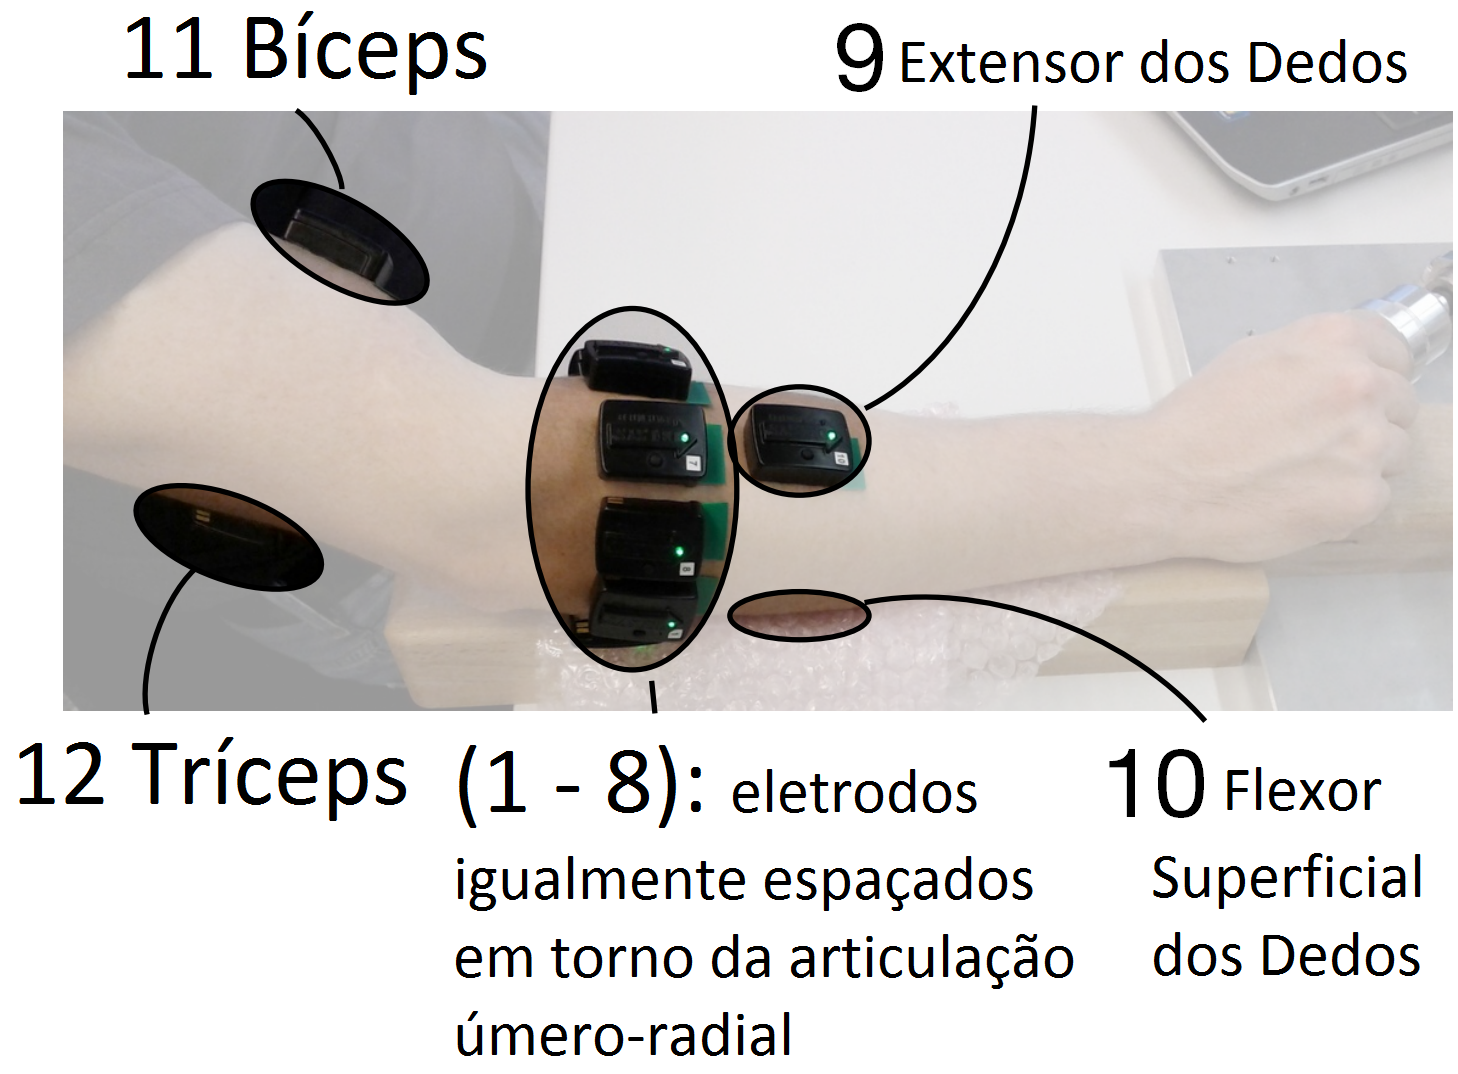
\includegraphics[width=0.75\linewidth]{./img/eletrodos.png}
	\end{center}
	\legend{Fonte: adaptado de \cite{Gijsberts2014}}
\end{figure}

%-------------------------------------------------------------------------
			\subsection{Sistema de Aquisição IEE}
%-------------------------------------------------------------------------
\textcolor{red}{TODO: descrever o \emph{hardware} utilizado na aquisição do IEE}.

%-------------------------------------------------------------------------
			\subsection{Realização de Movimentos}
%-------------------------------------------------------------------------
Após o posicionamento de eletrodos, os voluntários sentam-se em frente a um monitor e apoiam o braço direito de forma relaxada sobre uma superfície horizontal próxima à altura do cotovelo. O monitor exibe um vídeo com uma mão direita, digitalmente animada, realizando movimentos de interesse que devem ser mimicados pelos voluntários. A Figura \ref{fig:video} apresenta a mão digitalmente animada realizando alguns dos movimentos de interesse.

\begin{figure}[htb]
	\caption{\label{fig:video}Trechos do vídeo apresentado aos voluntários na aquisição do IEE.}
	\begin{center}
	    
\includegraphics[width=0.75\linewidth]{./img/placeholder.png}
	\end{center}
	%\legend{Fonte: adaptado de \cite{Gijsberts2014}}
\end{figure}

Primeiramente, realiza-se um ``treinamento'' com o voluntário, exibindo o vídeo e apresentando os movimentos que devem ser realizados (sem aquisição de sinal), de modo a reduzir possíveis erros na realização de movimentos para uma segunda exibição, quando os sinais de EMG serão devidamente adquiridos. Cada movimento apresentado em vídeo tem duração de 5 segundos, com um intervalo de 3 segundos de repouso entre movimentos. O voluntário realiza 6 repetições consecutivas para os 17 movimentos descritos na Tabela \ref{tab:movimentos}.

\begin{table}[htb]
	\begin{tabular}{m{0.5cm} m{1.5cm} m{2cm} | m{0.5cm} m{1.5cm} m{2cm} | m{0.5cm} m{1.5cm} m{2cm}}
		\toprule
		\# & Descrição & Imagem \newline demonstrativa	& \# & Descrição & Imagem \newline demonstrativa & \# & Descrição & Imagem \newline demonstrativa\\
		\midrule \midrule					
		1	&	Polegar esticado, flexão dos outros dedos.	& 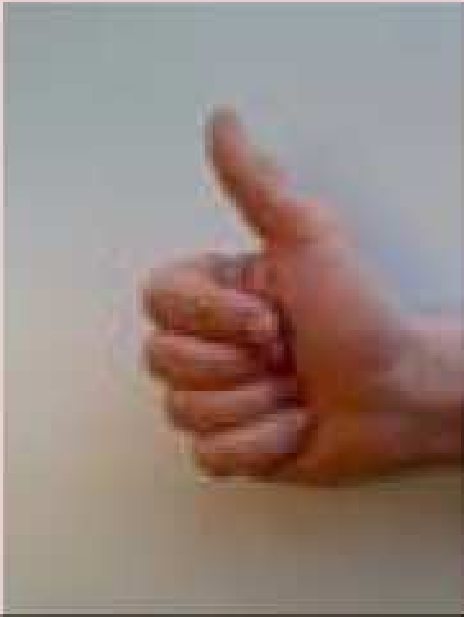
\includegraphics[width=\linewidth]{./img/moves/mov1.png} &
		2	&	Extensão do indicador e dedo médio, flexão dos outros dedos.	& 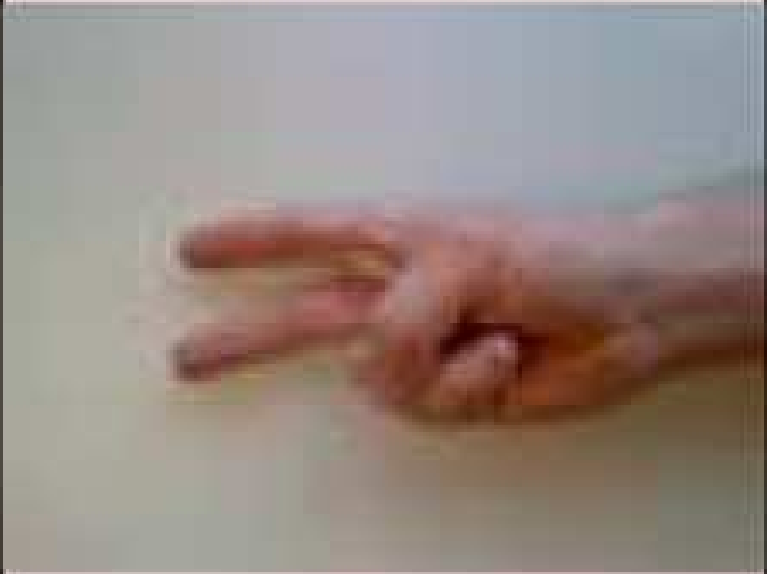
\includegraphics[width=\linewidth]{./img/moves/mov2.png} &
		3	&	Flexão do dedo anelar e mínimo, extensão dos outros dedos.	& 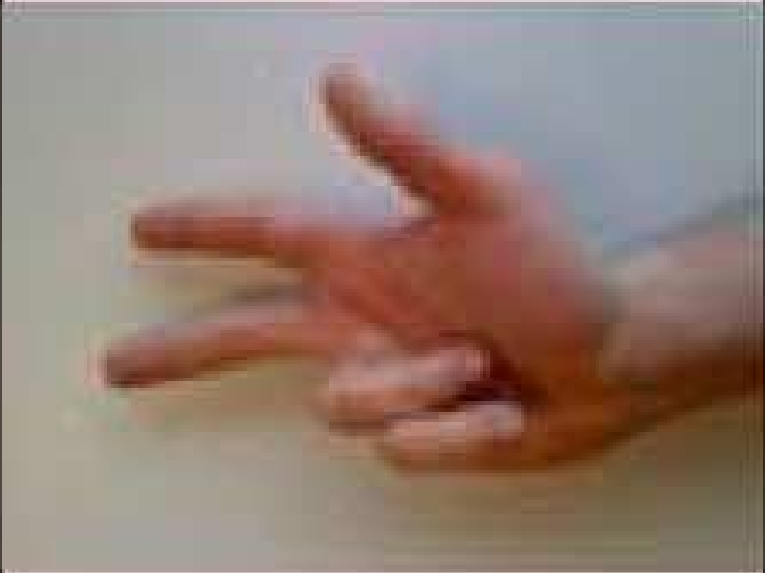
\includegraphics[width=\linewidth]{./img/moves/mov3.png}\\
		\midrule
		4	&	Polegar para a base do dedo mínimo.	& 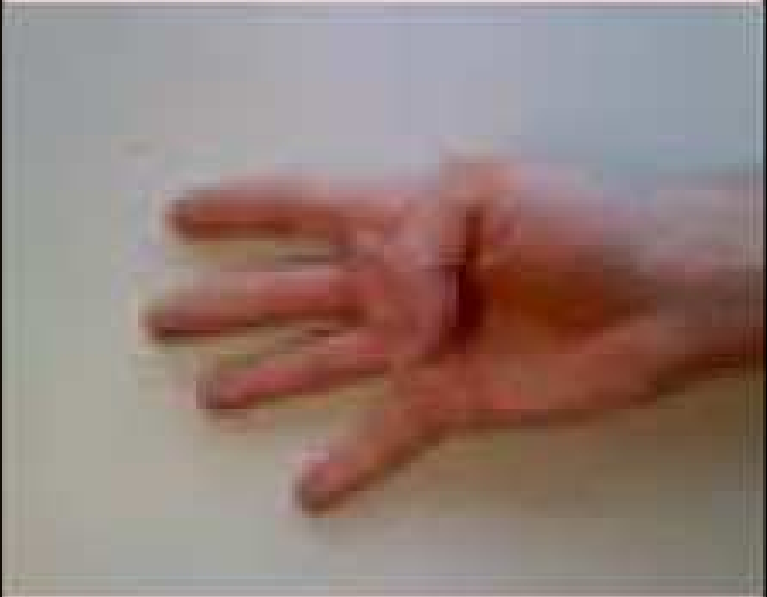
\includegraphics[width=\linewidth]{./img/moves/mov4.png} &
		5	&	Abdução (``afastamento'') de todos os dedos extendidos.	& 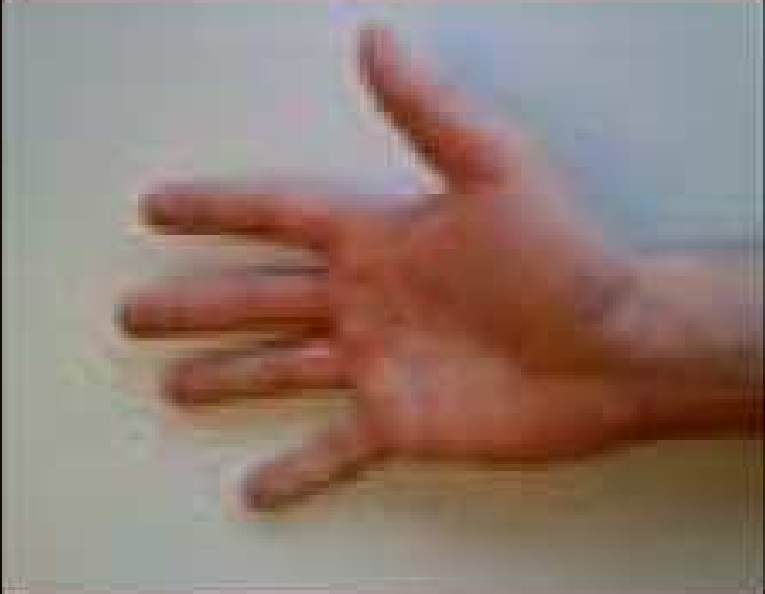
\includegraphics[width=\linewidth]{./img/moves/mov5.png} &
		6	&	Flexão de todos os dedos ao punho.	& 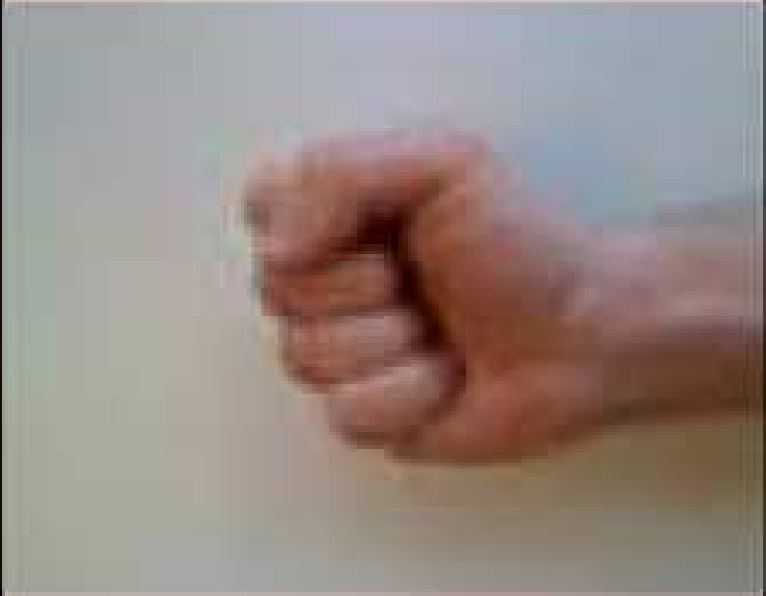
\includegraphics[width=\linewidth]{./img/moves/mov6.png}\\
		\midrule
		7	&	Extensão do indicador em movimento de ``apontar''.	& 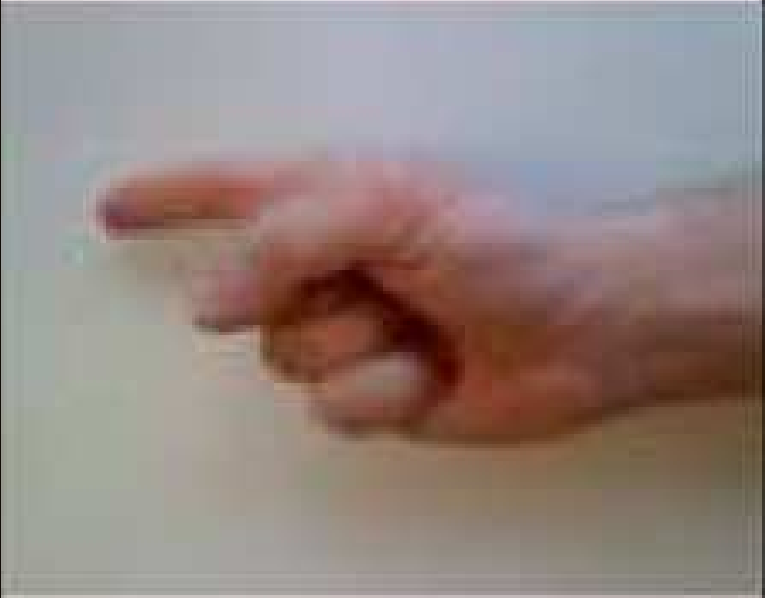
\includegraphics[width=\linewidth]{./img/moves/mov7.png} &
		8	&	Adução (``aproximação'') de todos os dedos extendidos.	& 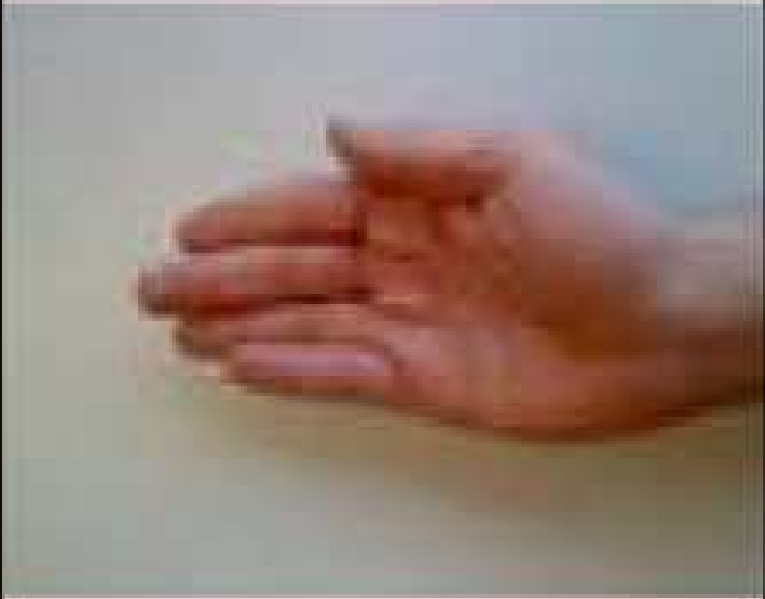
\includegraphics[width=\linewidth]{./img/moves/mov8.png} &
		9 10	&	Rotação de punho em torno do dedo médio, dois sentidos.	& 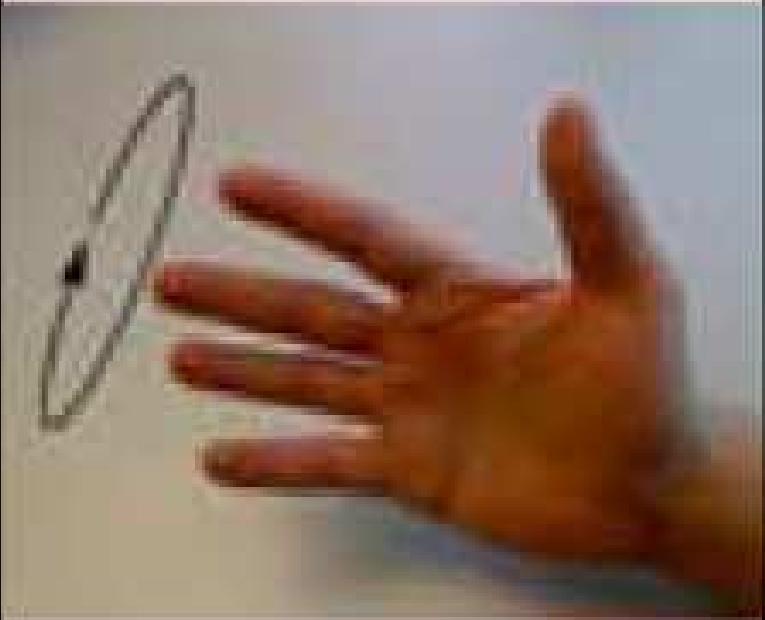
\includegraphics[width=\linewidth]{./img/moves/mov9.png} 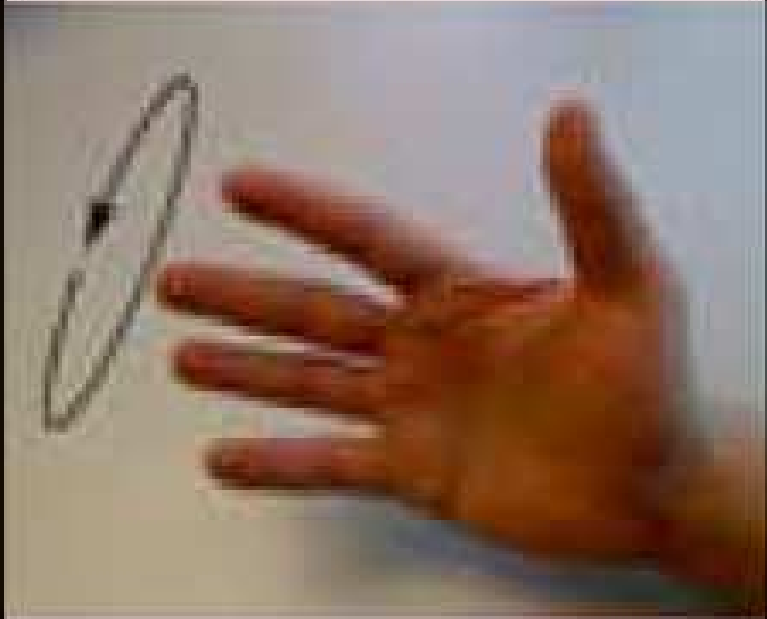
\includegraphics[width=\linewidth]{./img/moves/mov10.png} \\
		\midrule
		11 12	&	Rotação de punho em torno do dedo mínimo, dois sentidos.	& 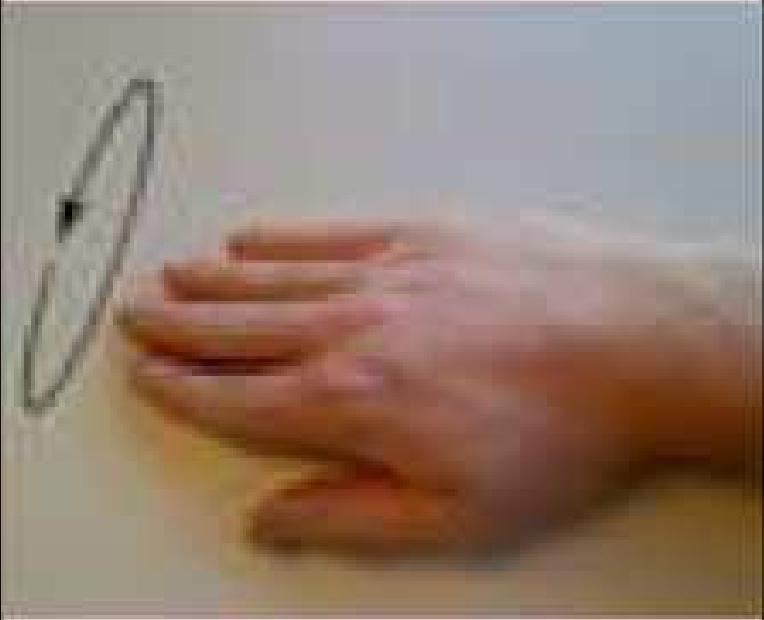
\includegraphics[width=\linewidth]{./img/moves/mov11.png} 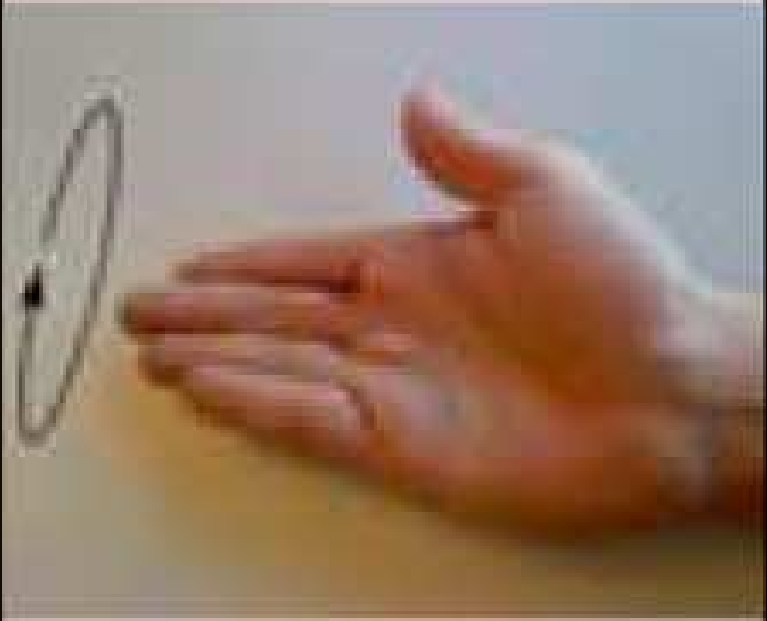
\includegraphics[width=\linewidth]{./img/moves/mov12.png} &
		13	&	Flexão de punho.	& 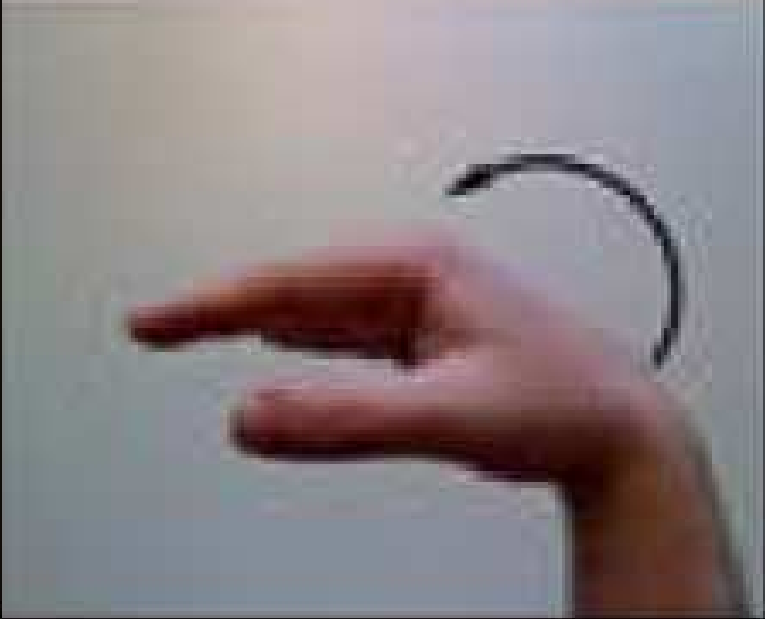
\includegraphics[width=\linewidth]{./img/moves/mov13.png} &
		14	&	Extensão de punho.	& 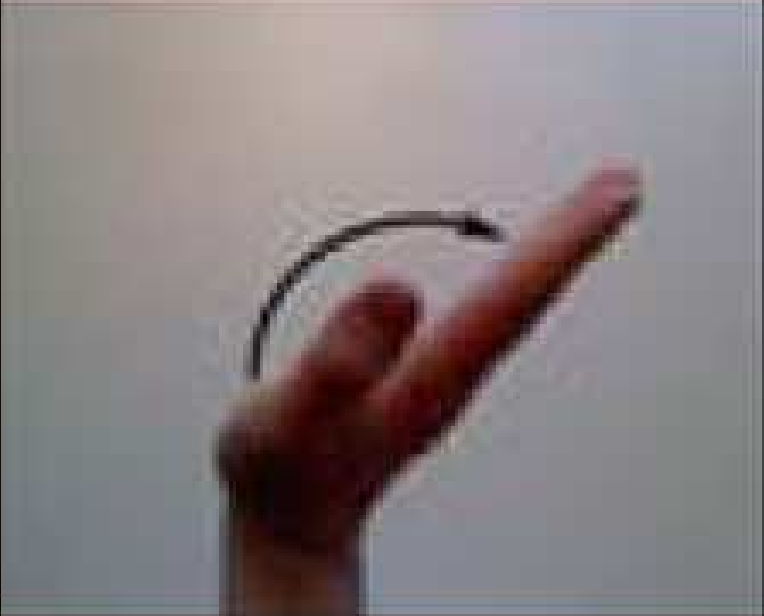
\includegraphics[width=\linewidth]{./img/moves/mov14.png}\\
		\midrule
		15	&	Desvio radial do punho.	& 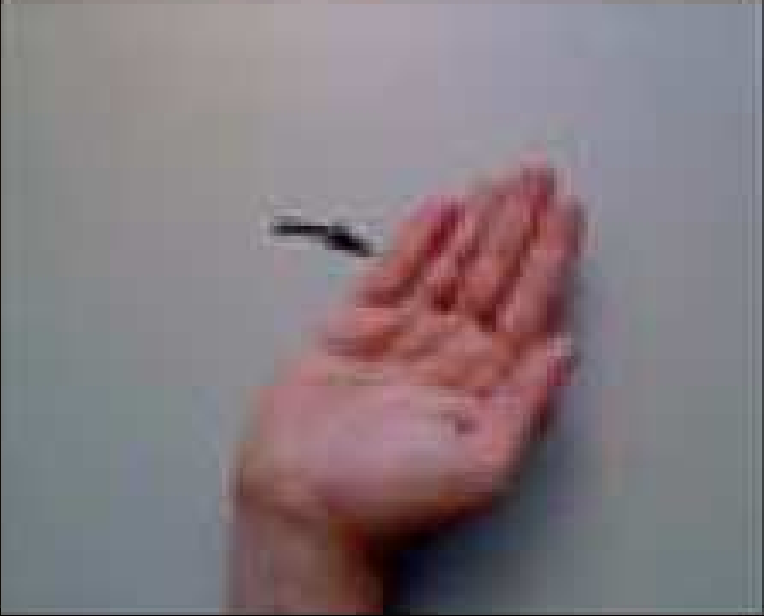
\includegraphics[width=\linewidth]{./img/moves/mov15.png} &
		16	&	Desvio ulnar do punho.	& 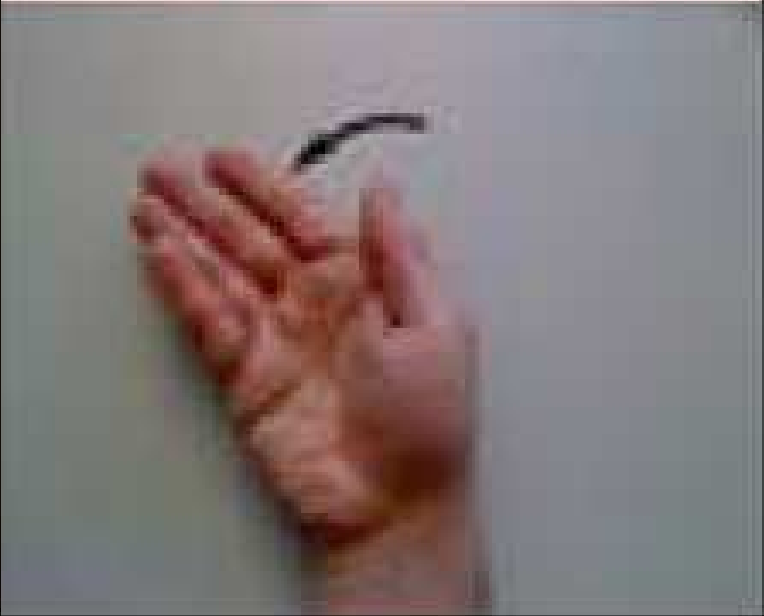
\includegraphics[width=\linewidth]{./img/moves/mov16.png} &
		17	&	Extensão de punho com mão cerrada.	& 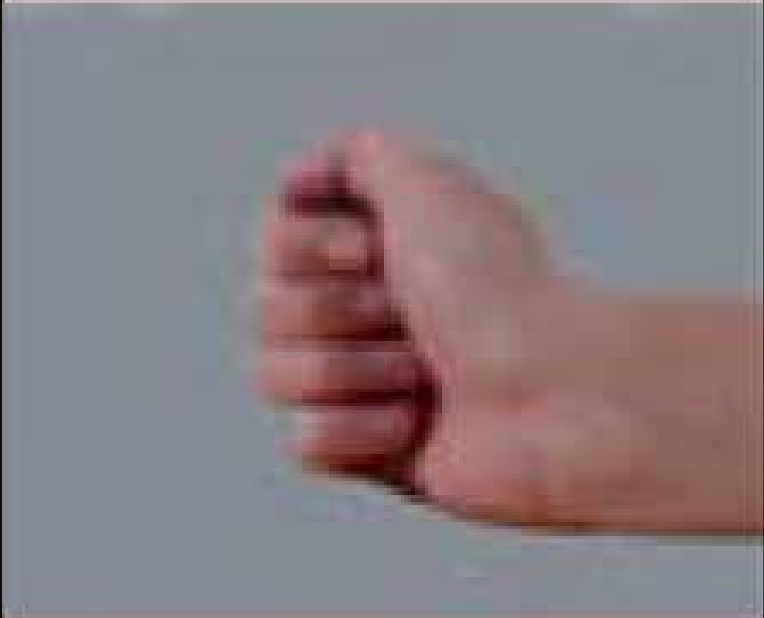
\includegraphics[width=\linewidth]{./img/moves/mov17.png}\\
		\bottomrule
	\end{tabular}
\end{table}


%=========================================================================
% METODOLOGIA EXPERIMENTAL
	\chapter{Metodologia Experimental}
%=========================================================================
		\section{Implementação de Métodos de Segmentação}
%-------------------------------------------------------------------------
Esta seção descreve a implementação dos métodos de segmentação desenvolvidos. O fluxograma da Figura \ref{flow:MTDs} apresenta de forma resumida os passos comuns aos quatro métodos, que serão explanados nas subseções seguintes. Os códigos em Matlab criados para os quatro métodos são apresentados nos Apêndices A - D.

% Set up a few colours
\colorlet{lcfree}{green}
\colorlet{lcnorm}{blue}
\colorlet{lccong}{red}
% -------------------------------------------------
% Set up a new layer for the debugging marks, and make sure it is on
% top
\pgfdeclarelayer{marx}
\pgfsetlayers{main,marx}
% A macro for marking coordinates (specific to the coordinate naming
% scheme used here). Swap the following 2 definitions to deactivate
% marks.
\providecommand{\cmark}[2][]{%
  \begin{pgfonlayer}{marx}
    \node [nmark] at (c#2#1) {#2};
  \end{pgfonlayer}{marx}
  } 
\providecommand{\cmark}[2][]{\relax} 
% -------------------------------------------------
% Start the picture
\begin{figure}[htb]
	\caption{\label{flow:MTDs} Diagrama de blocos geral para os métodos de segmentação MTD1 - MTD4.}
	\begin{center}
		\begin{tikzpicture}[%
			>=triangle 60,              % Nice arrows; your taste may be different
			start chain=going below,    % General flow is top-to-bottom
			node distance=6mm and 60mm, % Global setup of box spacing
			every join/.style={norm},   % Default linetype for connecting boxes
			]
		% ------------------------------------------------- 
		% A few box styles 
		% <on chain> *and* <on grid> reduce the need for manual relative
		% positioning of nodes
		\tikzset{
		  base/.style={draw, on chain, on grid, align=center, minimum height=4ex},
		  proc/.style={base, rectangle, text width=8em},
		  test/.style={base, diamond, aspect=2, text width=8em},
		  term/.style={proc, rounded corners},
		  % coord node style is used for placing corners of connecting lines
		  coord/.style={coordinate, on chain, on grid, node distance=6mm and 25mm},
		  % nmark node style is used for coordinate debugging marks
		  nmark/.style={draw, cyan, circle, font={\sffamily\bfseries}},
		  % -------------------------------------------------
		  % Connector line styles for different parts of the diagram
		  norm/.style={->, draw, lcnorm},
		  free/.style={->, draw, lcfree},
		  cong/.style={->, draw, lccong},
		  it/.style={font={\small\itshape}}
		}
		% -------------------------------------------------
		% Node placement: column 1
		\node [proc, fill=lcfree!25] (pre) {Preprocessamento (retificação e normalização)};
		\node [proc, fill=lcfree!25, right=of pre, xshift=-4em, join] (id) {Identificação de segmentos para cada canal utilizando MTD\#};
		\node [proc, fill=lcfree!25, right=of id, xshift=-4em, join] (dbscan) {Agrupamento de posições de segmentos utilizando DBSCAN};
		\node [proc, fill=lcfree!25, right=of dbscan, xshift=-4em, join] {Segmentação do sinal nas médias das posições agrupadas};
		% -------------------------------------------------
		\end{tikzpicture}
	\end{center}
\end{figure}


%-------------------------------------------------------------------------
			\subsection {Preprocessamento}
%-------------------------------------------------------------------------
				\subsubsection{Retificação Completa}
%-------------------------------------------------------------------------
Os sinais de eletromiografia para ambas as bases de dados (NinaPro e IEE) são armazenados mantendo sua polaridade original (i.e. amostras do sinal podem assumir valores positivos e negativos). Primeiramente, realiza-se a retificação completa dos sinais tomando o módulo dos valores amostrados (em Matlab, função \emph{abs()}). A retificação completa do sinal mantém sua energia e é fundamental para a implementação dos métodos de segmentação aqui desenvolvidos. A Figura \ref{fig:rectification} exemplifica o resultado esperado para a retificação completa de um trecho de sinal de eletromiografia.

\begin{figure}[htb]
	\caption{\label{fig:rectification} Retificação completa de trecho de sinal de eletromiografia.}
	\begin{center}
	    
\includegraphics[width=0.75\linewidth]{./img/placeholder.png}
	\end{center}
	%\legend{Fonte: adaptado de BASMAJIAN \& DE LUCA, 1985}
\end{figure}

%-------------------------------------------------------------------------
				\subsubsection{Normalização}
%-------------------------------------------------------------------------
Os sinais para cada canal de aquisição são normalizados de acordo com seu valor máximo, de modo que seu novo valor máximo seja unitário, a partir da equação \ref{eq:x_normalization}, onde $x$ é o sinal original para um canal e $x_{norm}$ é sua versão normalizada. A normalização de canais faz com que os parâmetros utilizados pelos métodos de segmentação sejam relativos ao valor máximo do sinal, possibilitando a implementação para diferentes voluntários. A Figura \ref{fig:normalization} exemplifica a normalização para três canais de um trecho de sinal já retificado.

\begin{equation}
	\label{eq:x_normalization}
	x_{norm} = \frac{x}{max(x)}
\end{equation}

\begin{figure}[htb]
	\caption{\label{fig:normalization}Normalização de canais de eletromiografia de acordo com seu valor máximo.}
	\begin{center}
	    
\includegraphics[width=0.75\linewidth]{./img/placeholder.png}
	\end{center}
	%\legend{Fonte: adaptado de BASMAJIAN \& DE LUCA, 1985}
\end{figure}

%-------------------------------------------------------------------------
			\subsection{Implementação dos Métodos de Segmentação}
%-------------------------------------------------------------------------
				\subsubsection{Parâmetros Utilizados}
%-------------------------------------------------------------------------
Cada método de segmentação MTD1 - MTD4 apresenta um conjunto de parâmetros ajustáveis. Tais parâmetros foram descritos anteriormentes na seção \ref{sec:MTDs}. Após investigações iniciais das segmentações obtidas com diferentes valores de parâmetros, fixou-se alguns destes parâmetros e realizou-se uma lista de valores a serem explorados na aplicação de cada método, a fim de obter os parâmetros mais adequados para as duas bases de dados utilizadas. A Tabela \ref{tab:combinacoes} apresenta os parâmetros ajustáveis de cada método e sua respectiva lista de valores explorados.

\begin{table}[htb]
\IBGEtab{\caption{\label{tab:combinacoes}Parâmetros ajustáveis para os métodos de segmentação.}}
{
	\begin{tabular}{cllc}
		\toprule
		Método 					& Parâmetros	& Valores utilizados						& Número total de combinações \\
		\midrule \midrule					
		\multirow{4}{*}{MTD1}	& $l$			& $10 \times 10^3$							& \multirow{4}{*}{16} \\
								& $r_{target}$	& $5,6 \times 10^{-5}$						& \\
								& $q$			& $[0.8 \quad 0.85 \quad 0.9 \quad 0.95]$	& \\
								& $T_{lim`}$	& $[0.05 \quad 0.1 \quad 0.15 \quad 0.2]$	& \\
		\midrule
		\multirow{4}{*}{MTD2}	& $l$			& $10 \times 10^3$							& \multirow{4}{*}{27} \\
								& $A$			& $[20 \quad 30 \quad 40]$					& \\
								& $B$			& $[2 \quad 5 \quad 8]$						& \\
								& $C$			& $[2 \quad 5 \quad 8]$						& \\
		\midrule					
		\multirow{3}{*}{MTD3}	& $W$			& TODO										& \multirow{3}{*}{TODO} \\
								& $B$			& TODO										& \\
								& $C$			& TODO										& \\
		\midrule					
		\multirow{2}{*}{MTD4}	& $W$			& TODO										& \multirow{2}{*}{TODO} \\
								& $T$			& TODO										& \\
		\bottomrule
	\end{tabular}
}{}
\end{table}


Para os métodos que utilizam parâmetro de comprimento de segmento $l$ (i.e. os métodos que produzem segmentos de comprimento de janela constante, MTD1 e MTD2) utilizou-se valor de $l$ como $10 \times 10^3$, que corresponde a 5 cinco segundos de aquisição para ambas as bases de dados (período de amostragem para ambas é de $500 \mu s$), sendo a mesma duração dos segmentos de vídeo mimicados pelos voluntários. O valor de MTD1 para $r_{target}$ foi obtido utilizando o código do Apêndice \ref{ap:r_target} como valor mínimo da razão entre número de segmentos e comprimento de sinal para a base de dados NinaPro.

%-------------------------------------------------------------------------
				\subsubsection{Identificação de segmentos utilizando \emph{k-means}}
%-------------------------------------------------------------------------
Os sinais para ambas as bases de dados são compostos por 12 canais de aquisição. Os métodos de segmentação são implementados individualmente aos doze canais. Para os métodos MTD1 e MTD2, as posições centrais dos segmentos obtidas em cada canal são armazenadas, enquanto que para os métodos MTD3 e MT4 armazena-se as posições de BEPs e EEPs. Tais posições são agrupadas utilizando o método de \emph{clustering k-means}. Este agrupamento permite a identificação dos segmentos obtidos nos diferentes canais que referem-se a um mesmo trecho de aumento da atividade muscular. Tomando a média de cada grupo, o sinal original pode então ser segmentado, de forma que os segmentos mantém coerência temporal entre canais. A Figura \ref{fig:kmeans1} exemplifica o grupamento das posições centrais de segmentos nos métodos MTD1 e MTD2 e a Figura \ref{fig:kmeans2} exemplifica o grupamento de BEPs e EEPs nos métodos MTD3 e MTD4.

\begin{figure}[htb]
	\caption{\label{fig:kmeans1}\emph{Clustering} por \emph{k-means} dos centros de segmentos obtidos pelos métodos MTD1 e MTD2.}
	\begin{center}
	    
\includegraphics[width=0.75\linewidth]{./img/placeholder.png}
	\end{center}
	%\legend{Fonte: adaptado de BASMAJIAN \& DE LUCA, 1985}
\end{figure}

\begin{figure}[htb]
	\caption{\label{fig:kmeans2}\emph{Clustering} por \emph{k-means} de BEPs e EEPs de segmentos obtidos pelos métodos MTD3 e MTD4.}
	\begin{center}
	    
\includegraphics[width=0.75\linewidth]{./img/placeholder.png}
	\end{center}
	%\legend{Fonte: adaptado de BASMAJIAN \& DE LUCA, 1985}
\end{figure}

%-------------------------------------------------------------------------
		\section{Rede Neural Artificial}
%-------------------------------------------------------------------------
Esta seção descreve a utilização de RNA para classificação dos segmentos obtidos de acordo com movimentos de interesse. O processo de classificação é representado pelo fluxograma da Figura \ref{flow:RNAresumo}, que será explanado nas subseções seguintes.

% Set up a few colours
\colorlet{lcfree}{green}
\colorlet{lcnorm}{blue}
\colorlet{lccong}{red}
% -------------------------------------------------
% Set up a new layer for the debugging marks, and make sure it is on
% top
\pgfdeclarelayer{marx}
\pgfsetlayers{main,marx}
% A macro for marking coordinates (specific to the coordinate naming
% scheme used here). Swap the following 2 definitions to deactivate
% marks.
\providecommand{\cmark}[2][]{%
  \begin{pgfonlayer}{marx}
    \node [nmark] at (c#2#1) {#2};
  \end{pgfonlayer}{marx}
  } 
\providecommand{\cmark}[2][]{\relax} 
% -------------------------------------------------
% Start the picture
\begin{figure}[htb]
	\caption{\label{flow:RNAs} Fluxograma da classificação de movimentos com RNAs.}
	\begin{center}
		\begin{tikzpicture}[%
			>=triangle 60,              % Nice arrows; your taste may be different
			start chain=going below,    % General flow is top-to-bottom
			node distance=6mm and 60mm, % Global setup of box spacing
			every join/.style={norm},   % Default linetype for connecting boxes
			]
		% ------------------------------------------------- 
		% A few box styles 
		% <on chain> *and* <on grid> reduce the need for manual relative
		% positioning of nodes
		\tikzset{
		  base/.style={draw, on chain, on grid, align=center, minimum height=4ex},
		  proc/.style={base, rectangle, text width=8em},
		  test/.style={base, diamond, aspect=2, text width=8em},
		  term/.style={proc, rounded corners},
		  % coord node style is used for placing corners of connecting lines
		  coord/.style={coordinate, on chain, on grid, node distance=6mm and 25mm},
		  % nmark node style is used for coordinate debugging marks
		  nmark/.style={draw, cyan, circle, font={\sffamily\bfseries}},
		  % -------------------------------------------------
		  % Connector line styles for different parts of the diagram
		  norm/.style={->, draw, lcnorm},
		  free/.style={->, draw, lcfree},
		  cong/.style={->, draw, lccong},
		  it/.style={font={\small\itshape}}
		}
		% -------------------------------------------------
		% Node placement: column 1
		\node [term, densely dotted, it, fill=lccong!25] (init) {INÍCIO};
		\node [proc, fill=lcfree!25, right=of init, xshift=-4em, join] (pre) {Segmentar o sinal com o MTD\#};
		\node [proc, fill=lcfree!25, right=of pre, xshift=-4em, join] (id) {Identificação de movimento associado a cada segmento (vetor de respostas)};
		\node [proc, fill=lcfree!25, right=of id, xshift=-4em, join] (dbscan) {Extração de características dos segmentos};
		\node [proc, fill=lcfree!25, join] (sep) {Separação de segmentos em grupos para treino, validação e teste};
		\node [proc, fill=lcfree!25, join, left=of sep, xshift=2em] (train) {Treinamento da RNA};
		\node [proc, fill=lcfree!25, join, left=of train, xshift=2em] {Obtenção de resultados de para todos os segmentos};
		% -------------------------------------------------
		\end{tikzpicture}
	\end{center}
\end{figure}


%-------------------------------------------------------------------------
			\subsection{Características Utilizadas como Preditores}
%-------------------------------------------------------------------------
Os preditores (``entradas'') utilizados pela RNA são o valor RMS, a variância e a frequência mediana do espectro de potência dos segmentos de sinal obtidos pelos métodos MTD1 - MTD4. Tais características foram selecionados de acordo com outros trabalhos já realizados no laboratório de Instrumentação Eletro-Eletrônica que obtiveram bons resultado para uso com RNA, como \cite{Favieiro2009}, \cite{Schons2014} e \cite{CeneXXXX}.

O valor RMS ou \emph{root mean square} de um sinal discreto \emph{x} de comprimento $L$ (em Matlab, função \emph{rms()}) é dada pela equação \ref{eq:rms} e a variância deste sinal (em Matlab, função \emph{var()}) é dada pela equação \ref{eq:var}, onde $\bar{x}$ é o valor médio do sinal. A frequência mediana é tal que a soma total da densidade de potência para frequências abaixo da frequência mediana é igual à soma total da densidade de potência para frequências acima da frequência mediana, sendo estimada pela função \emph{medfreq()} em Matlab.

\begin{equation}
	\label{eq:rms}
	rms(x) = \sqrt{\frac{1}{L}\sum\limits_{i=1}^{L}x_i^2} 
\end{equation}

\begin{equation}
	\label{eq:var}
	var(x) = \frac{1}{L-1}\sum\limits_{i=1}^{L}(x_i - \bar{x})^2
\end{equation}

%-------------------------------------------------------------------------
			\subsection{Movimentos Utilizados como Alvo}
%-------------------------------------------------------------------------
Obtém-se os movimentos associados a cada segmento obtido a partir de sua posição temporal no sinal original, já que durante a aquisição de dados os movimentos são realizados na mesma sequência para todos os voluntários. A base de dados NinaPro apresenta um vetor \emph{stimulus} que indica os instantes em que foram apresentados cada movimento a ser replicado pelo volunário. A partir deste vetor e das posições dos segmentos dentro do sinal original, utiliza-se o código apresentado no Apêndice \ref{ap:idMoves} para criar a variável que servirá como resposta esperada no treinamento da RNA. 


%=========================================================================
% RESULTADOS E DISCUSSÕES
	\chapter{Resultados e Discussões}
%=========================================================================

%=========================================================================
% CONCLUSÃO
	\chapter{Conclusões}
%=========================================================================

%=========================================================================
% PROPOSTA DE TRABALHOS FUTUROS
	\chapter{Propostas de Futuros Trabalhos}
%=========================================================================

%=========================================================================
% REFERÊNCIAS BIBLIOGRÁFICAS
	\postextual
	\bibliography{referencias.bib}
%=========================================================================

%=========================================================================
% APÊNDICES
	\begin{apendicesenv}
	\partapendices
%=========================================================================
\chapter{Função em Matlab para MTD1}
\lstinputlisting{../../matlab/seg_mtd1.m}
%-------------------------------------------------------------------------
\chapter{Função em Matlab para MTD2}
\lstinputlisting{../../matlab/seg_mtd2.m}
%-------------------------------------------------------------------------
%\chapter{Função em Matlab para MTD3}
%\lstinputlisting{../../matlab/seg_mtd3.m}
%%-------------------------------------------------------------------------
%\chapter{Função em Matlab para MTD4}
%\lstinputlisting{../../matlab/seg_mtd4.m}
%-------------------------------------------------------------------------
\chapter{Código utilizado para determinação de $r_{target}$ do MTD1}
\label{ap:r_target}
\lstinputlisting{../../matlab/rtarget_mtd1.m}
%-------------------------------------------------------------------------
\chapter{Função em Matlab para obtenção dos movimentos relacionados aos segmentos}
\label{ap:idMoves}
\lstinputlisting{../../matlab/identifyClasses.m}
%-------------------------------------------------------------------------
\end{apendicesenv}

\end{document}
